\documentclass[12pt]{article}
\usepackage{preamble}
\usepackage{longtable}

\geometry{a4paper, left=2.5cm, right=2.5cm, top=2cm, bottom=2.5cm}

\pagestyle{plain}

\newcommand{\placeholder}[1]{{\color{magenta}#1}}

\chead{
    \begin{minipage}{1\linewidth}
        \begin{wrapfigure}{r}{0pt}
            
\includegraphics[height=1cm]{images/logo}
        \end{wrapfigure}
        {
            \centering
            \sffamily\scriptsize
            \textbf{
                Санкт-Петербургский национальный исследовательский университет \\
                информационных технологий, механики и оптики}
            %th3p4g
            \vspace{2mm}

            \quad\quad\quad\quad\quad\quad\ \textbf{УЧЕБНЫЙ ЦЕНТР ОБЩЕЙ ФИЗИКИ ФТФ}
        }
    \end{minipage}
}



\begin{document}
    \vspace*{2\baselineskip}

    \thispagestyle{fancy}

    \noindent
    \textbf{Группа} \underline{\hspace{4.85cm}} \hfill \textbf{К работе допущен} \underline{\hspace{4cm}} \\[0.5cm]
    \textbf{Студент} \underline{\hspace{4.6cm}} \hfill \textbf{Работа выполнена} \underline{\hspace{4cm}} \\[0.5cm]
    \textbf{Преподаватель} \underline{\hspace{3.2cm}} \hfill \textbf{Отчет принят} \underline{\hspace{4.85cm}} \\


    \begin{center}
    {\huge \textbf{Рабочий протокол и отчёт по\\ лабораторной работе № \placeholder{X.YZ}}}

        \smallvspace

        {\Large \placeholder{Название лабораторной работы}}
    \end{center}


    \noindent
    1. \textbf{Цель работы.}

    \begin{enumerate}
        \item \placeholder{Цель №1}

        \item \placeholder{Цель №N}
    \end{enumerate}

    \mediumvspace

    \noindent
    2. \textbf{Задачи, решаемые при выполнении работы.}

    \begin{enumerate}
        \item \placeholder{Задача №1}

        \item \placeholder{Задача №2}

        \item \placeholder{Задача №N}
    \end{enumerate}

    \mediumvspace

    \noindent
    3. \textbf{Объект исследования: } \placeholder{Объект исследования}

    \mediumvspace

    \noindent
    4. \textbf{Метод экспериментального исследования.}

    \placeholder{Метод исследования}

    \mediumvspace

    \noindent
    5. \textbf{Рабочие формулы и исходные данные.}

    \placeholder{Рабочая формула №1:
\[
\vec{F} = m\vec{a}
\]

Рабочая формула №2:
\[
E = mc^2
\]}

    \mediumvspace

    \clearpage

    \noindent
    6. \textbf{Измерительные приборы.}

    \smallvspace

    \begin{center}
    \begin{tabular}{|c|m{4cm}|C{2cm}|C{3cm}|c|}
        \hline
        № п/п & Наименование            & Предел\newlineизмерений & Цена\newlineделения    & $\Delta_{\text{и}}$ \\
        \hline
        1     & Амперметр               & 20 мА                   & 0.01 \text{мА/дел}                     & 0.01 \text{мА}     \\
        \hline
        2     & Вольтметр               & 20 В                    & 0.01 \text{В/дел}                      & 0.01 \text{В}      \\
        \hline

    \end{tabular}

    \smallvspace

    \textit{Таблица 1.} Измерительные приборы
\end{center}

    \mediumvspace

    7. \textbf{Схема установки. (перечень схем, которые составляют Приложение 1).}

    \hyperlink{schema1}{Схема установки} прилагается в Приложении 1

    \mediumvspace

    8. \textbf{Результаты прямых измерений и их обработки (таблицы, примеры расчетов).}

    \begin{itemize}
    \item Прилагается \hyperlink{table2}{Таблица 2} в Приложении 2
\end{itemize}


    \mediumvspace

    9. \textbf{Расчет результатов косвенных измерений (таблицы, примеры расчетов).}

    \begin{itemize}
    \item \placeholder{Интересные вычисления: $E = 0.4 \cdot (3 \cdot 10^8)^2 = 3.6 \cdot 10^{16}$}

    \item Прилагается \hyperlink{tableM}{Таблица M} в Приложении 2
\end{itemize}

    \mediumvspace

    10. \textbf{Расчёт погрешности измерений.}

    \mediumvspace

    11. \textbf{Графики (перечень графиков, которые составляют Приложение 3).}

    \hyperlink{diagram1}{График 1} прилагаются в Приложении 3

    \mediumvspace

    12. \textbf{Окончательные результаты.}

    \text{Доверительный интервал для значения внутреннего сопротивления:}
\[
r = (6.7635000 \pm 0.0000014) \cdot 10^{-1} \ \frac{\text{В}}{\text{мА}} \quad \varepsilon_r = 2.0148 \cdot 10^{-5} \%
\]

\text{Доверительный интервал для значения ЭДС источника:}
\[
\mathcal{E} = (10.553770 \pm 0.000010) \ \text{В} \quad \varepsilon_\mathcal{E} = 4.549 \cdot 10^{-5} \%
\]

\text{Значение тока, при котором достигается максимум значения полезной мощности:}
\[
I^* = 7.51 \ \text{мА} \quad P_{Rmax} = 41.15 \ \text{мВт}
\]

\text{Режим согласования:}
\[
R_{согл} = 0.73 \ \frac{\text{В}}{\text{мА}} \approx r
\]

\text{Проверка значения силы тока при КПД = 0.5}:
\[
I_{\eta = 0.5}^* = 7.80 \ \text{мА} \quad \Delta I^* = |I^* - I_{\eta = 0.5}^*| = 0.29 \ \text{мА}
\]

    \mediumvspace

    13. \textbf{Выводы и анализ результатов работы.}

    \placeholder{На основе результатов вышло пу-пу-пу}

    \clearpage

    \begin{center}
        \LARGE
        \textbf{Приложение 1. Схема установки}
    \end{center}

    \mediumvspace

    \hypertarget{schema1}{}

\begin{center}
    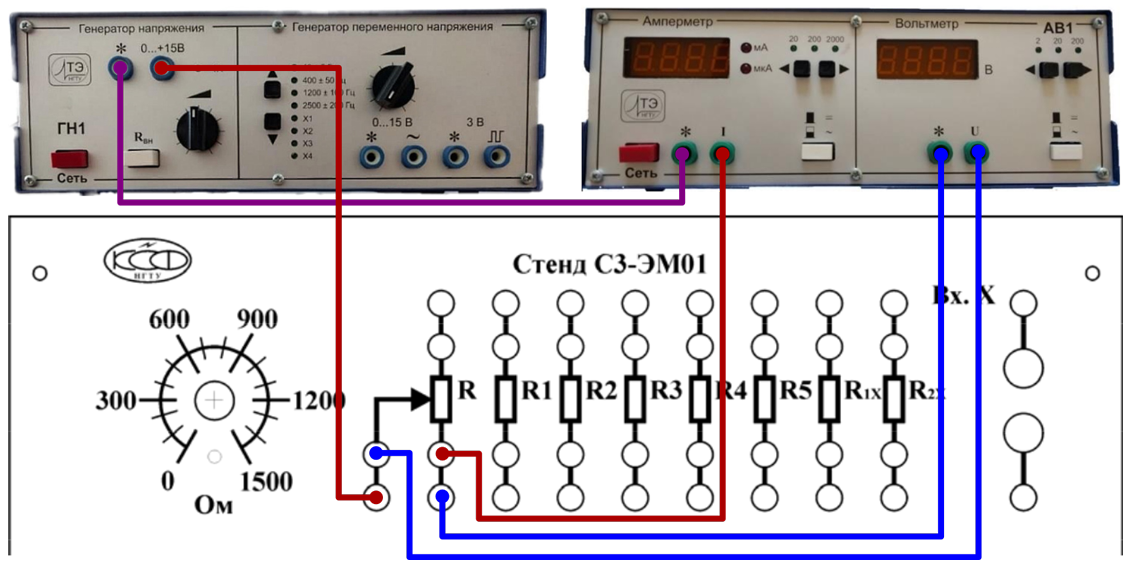
\includegraphics[width=15cm]{images/schema1}

    \smallvspace

    \textit{Рисунок 1.} Схема соединений источника, измерительных приборов и
    измерительного стенда
\end{center}






    \clearpage

    \begin{center}
        \LARGE
        \textbf{Приложение 2. Таблицы измерений и расчётов}
    \end{center}

    \mediumvspace

    \begin{center}
    \hypertarget{tableN}{}

    \renewcommand{\arraystretch}{1.8}

    \begin{tabular}{|C{3cm}|C{3cm}|C{3cm}|C{3cm}|}
        \hline
        \placeholder{$x$, м}            & \placeholder{$y$, м}     & \placeholder{$z$, мм}       & \placeholder{$w$ кг}    \\
        \hline
        \placeholder{$0.520 \pm 0.705$} & \placeholder{$1.890 \pm 0.005$} & \placeholder{$78.0 \pm 0.9$} & \placeholder{$367.0 \pm 0.5$} \\
        \hline
    \end{tabular}

    \smallvspace

    \textit{Таблица \placeholder{N}.} \placeholder{Какие-то забавные измерения}
\end{center}

    \begin{center}
    \hypertarget{table3}{}

    \renewcommand{\arraystretch}{1.8}

    \begin{tabular}{|c|C{2.5cm}|C{2.5cm}|C{1.8cm}|}
        \hline
         & \placeholder{$x - y$, м} & \placeholder{$2x - y$, м} & \placeholder{$\displaystyle \sqrt{\frac{a}{b}}$, с}  \\
        \hline
        1 & \placeholder{$0.540 \pm 0.065$}   & \placeholder{$0.840 \pm 0.500$}   & \placeholder{$7.5 \pm 1.1$}                       \\
        \hline
    \end{tabular}

    \smallvspace

    \textit{Таблица \placeholder{M}.} \placeholder{Какие-то интересные расчёты}

\end{center}

    \clearpage

    \begin{center}
        \LARGE
        \textbf{Приложение 3. Графики}
    \end{center}

    \mediumvspace

    \hypertarget{diagram1}{}

\begin{center}
    
\includegraphics[width=15cm]{images/logo}

    \smallvspace

    \textit{График 1.} Зависимость $U(I) = \mathscr{E} - Ir$
\end{center}

\begin{center}
    
\includegraphics[width=15cm]{images/logo}

    \smallvspace

    \textit{График 2.} Мощности $P, P_R, P_S$
\end{center}

\begin{center}
    
\includegraphics[width=15cm]{images/logo}

    \smallvspace

    \textit{График 3.} Зависимость КПД $\eta = \frac{P_R}{P}$
\end{center}



\end{document}